\documentclass[twoside]{book}

% Packages required by doxygen
\usepackage{fixltx2e}
\usepackage{calc}
\usepackage{doxygen}
\usepackage[export]{adjustbox} % also loads graphicx
\usepackage{graphicx}
\usepackage[utf8]{inputenc}
\usepackage{makeidx}
\usepackage{multicol}
\usepackage{multirow}
\PassOptionsToPackage{warn}{textcomp}
\usepackage{textcomp}
\usepackage[nointegrals]{wasysym}
\usepackage[table]{xcolor}

% Font selection
\usepackage[T1]{fontenc}
\usepackage[scaled=.90]{helvet}
\usepackage{courier}
\usepackage{amssymb}
\usepackage{sectsty}
\renewcommand{\familydefault}{\sfdefault}
\allsectionsfont{%
  \fontseries{bc}\selectfont%
  \color{darkgray}%
}
\renewcommand{\DoxyLabelFont}{%
  \fontseries{bc}\selectfont%
  \color{darkgray}%
}
\newcommand{\+}{\discretionary{\mbox{\scriptsize$\hookleftarrow$}}{}{}}

% Page & text layout
\usepackage{geometry}
\geometry{%
  a4paper,%
  top=2.5cm,%
  bottom=2.5cm,%
  left=2.5cm,%
  right=2.5cm%
}
\tolerance=750
\hfuzz=15pt
\hbadness=750
\setlength{\emergencystretch}{15pt}
\setlength{\parindent}{0cm}
\setlength{\parskip}{3ex plus 2ex minus 2ex}
\makeatletter
\renewcommand{\paragraph}{%
  \@startsection{paragraph}{4}{0ex}{-1.0ex}{1.0ex}{%
    \normalfont\normalsize\bfseries\SS@parafont%
  }%
}
\renewcommand{\subparagraph}{%
  \@startsection{subparagraph}{5}{0ex}{-1.0ex}{1.0ex}{%
    \normalfont\normalsize\bfseries\SS@subparafont%
  }%
}
\makeatother

% Headers & footers
\usepackage{fancyhdr}
\pagestyle{fancyplain}
\fancyhead[LE]{\fancyplain{}{\bfseries\thepage}}
\fancyhead[CE]{\fancyplain{}{}}
\fancyhead[RE]{\fancyplain{}{\bfseries\leftmark}}
\fancyhead[LO]{\fancyplain{}{\bfseries\rightmark}}
\fancyhead[CO]{\fancyplain{}{}}
\fancyhead[RO]{\fancyplain{}{\bfseries\thepage}}
\fancyfoot[LE]{\fancyplain{}{}}
\fancyfoot[CE]{\fancyplain{}{}}
\fancyfoot[RE]{\fancyplain{}{\bfseries\scriptsize 制作者 Doxygen }}
\fancyfoot[LO]{\fancyplain{}{\bfseries\scriptsize 制作者 Doxygen }}
\fancyfoot[CO]{\fancyplain{}{}}
\fancyfoot[RO]{\fancyplain{}{}}
\renewcommand{\footrulewidth}{0.4pt}
\renewcommand{\chaptermark}[1]{%
  \markboth{#1}{}%
}
\renewcommand{\sectionmark}[1]{%
  \markright{\thesection\ #1}%
}

% Indices & bibliography
\usepackage{natbib}
\usepackage[titles]{tocloft}
\setcounter{tocdepth}{3}
\setcounter{secnumdepth}{5}
\makeindex

% Hyperlinks (required, but should be loaded last)
\usepackage{ifpdf}
\ifpdf
  \usepackage[pdftex,pagebackref=true]{hyperref}
\else
  \usepackage[ps2pdf,pagebackref=true]{hyperref}
\fi
\hypersetup{%
  colorlinks=true,%
  linkcolor=blue,%
  citecolor=blue,%
  unicode%
}

% Custom commands
\newcommand{\clearemptydoublepage}{%
  \newpage{\pagestyle{empty}\cleardoublepage}%
}

\usepackage{caption}
\captionsetup{labelsep=space,justification=centering,font={bf},singlelinecheck=off,skip=4pt,position=top}

%===== C O N T E N T S =====

\begin{document}

% Titlepage & ToC
\hypersetup{pageanchor=false,
             bookmarksnumbered=true,
             pdfencoding=unicode
            }
\pagenumbering{alph}
\begin{titlepage}
\vspace*{7cm}
\begin{center}%
{\Large Qc\+Ps\+Ratio2\+Ma \\[1ex]\large 1.\+0 }\\
\vspace*{1cm}
{\large 制作者 Doxygen 1.8.14}\\
\end{center}
\end{titlepage}
\clearemptydoublepage
\pagenumbering{roman}
\tableofcontents
\clearemptydoublepage
\pagenumbering{arabic}
\hypersetup{pageanchor=true}

%--- Begin generated contents ---
\chapter{结构体索引}
\section{结构体}
这里列出了所有结构体,并附带简要说明\+:\begin{DoxyCompactList}
\item\contentsline{section}{\mbox{\hyperlink{struct_interval}{Interval}} \\*表示一个区间 }{\pageref{struct_interval}}{}
\end{DoxyCompactList}

\chapter{文件索引}
\section{文件列表}
这里列出了所有文件,并附带简要说明\+:\begin{DoxyCompactList}
\item\contentsline{section}{Q\+C\+P\+S\+Ratio2\+Ma/includes/\mbox{\hyperlink{_ma_calculate_8h}{Ma\+Calculate.\+h}} \\*对\+Ma\+Calculate.\+c中使用的函数及结构体进行声明 }{\pageref{_ma_calculate_8h}}{}
\item\contentsline{section}{Q\+C\+P\+S\+Ratio2\+Ma/includes/\mbox{\hyperlink{main_8h}{main.\+h}} \\*对main.\+c中使用的函数进行声明 }{\pageref{main_8h}}{}
\item\contentsline{section}{Q\+C\+P\+S\+Ratio2\+Ma/includes/\mbox{\hyperlink{_ratio_calculate_8h}{Ratio\+Calculate.\+h}} \\*对\+Ratio\+Calculate.\+c中使用的函数进行声明 }{\pageref{_ratio_calculate_8h}}{}
\item\contentsline{section}{Q\+C\+P\+S\+Ratio2\+Ma/includes/\mbox{\hyperlink{_type_and_consts_8h}{Type\+And\+Consts.\+h}} \\*定义类型及常数 }{\pageref{_type_and_consts_8h}}{}
\item\contentsline{section}{Q\+C\+P\+S\+Ratio2\+Ma/src/\mbox{\hyperlink{_ma_calculate_8c}{Ma\+Calculate.\+c}} \\*根据动静压比计算马赫数 }{\pageref{_ma_calculate_8c}}{}
\item\contentsline{section}{Q\+C\+P\+S\+Ratio2\+Ma/src/\mbox{\hyperlink{main_8c}{main.\+c}} \\*程序运行起始文件 }{\pageref{main_8c}}{}
\item\contentsline{section}{Q\+C\+P\+S\+Ratio2\+Ma/src/\mbox{\hyperlink{_ratio_calculate_8c}{Ratio\+Calculate.\+c}} \\*计算动静压比值 }{\pageref{_ratio_calculate_8c}}{}
\end{DoxyCompactList}

\chapter{结构体说明}
\hypertarget{struct_interval}{}\section{Interval结构体 参考}
\label{struct_interval}\index{Interval@{Interval}}


表示一个区间.  




{\ttfamily \#include $<$Ma\+Calculate.\+h$>$}

\subsection*{成员变量}
\begin{DoxyCompactItemize}
\item 
\mbox{\hyperlink{_type_and_consts_8h_a3f1431cb9f76da10f59246d1d743dc2c}{Float64}} \mbox{\hyperlink{struct_interval_a32be7f9967586b049961daa00b62069c}{start}}
\begin{DoxyCompactList}\small\item\em 区间左端点 \end{DoxyCompactList}\item 
\mbox{\hyperlink{_type_and_consts_8h_a3f1431cb9f76da10f59246d1d743dc2c}{Float64}} \mbox{\hyperlink{struct_interval_a9d014ab0dd1707f6c5d2a70370746263}{end}}
\begin{DoxyCompactList}\small\item\em 区间右端点 \end{DoxyCompactList}\end{DoxyCompactItemize}


\subsection{详细描述}
表示一个区间. 

\subsection{结构体成员变量说明}
\mbox{\Hypertarget{struct_interval_a9d014ab0dd1707f6c5d2a70370746263}\label{struct_interval_a9d014ab0dd1707f6c5d2a70370746263}} 
\index{Interval@{Interval}!end@{end}}
\index{end@{end}!Interval@{Interval}}
\subsubsection{\texorpdfstring{end}{end}}
{\footnotesize\ttfamily \mbox{\hyperlink{_type_and_consts_8h_a3f1431cb9f76da10f59246d1d743dc2c}{Float64}} end}



区间右端点 

\mbox{\Hypertarget{struct_interval_a32be7f9967586b049961daa00b62069c}\label{struct_interval_a32be7f9967586b049961daa00b62069c}} 
\index{Interval@{Interval}!start@{start}}
\index{start@{start}!Interval@{Interval}}
\subsubsection{\texorpdfstring{start}{start}}
{\footnotesize\ttfamily \mbox{\hyperlink{_type_and_consts_8h_a3f1431cb9f76da10f59246d1d743dc2c}{Float64}} start}



区间左端点 



该结构体的文档由以下文件生成\+:\begin{DoxyCompactItemize}
\item 
Q\+C\+P\+S\+Ratio2\+Ma/includes/\mbox{\hyperlink{_ma_calculate_8h}{Ma\+Calculate.\+h}}\end{DoxyCompactItemize}

\chapter{文件说明}
\hypertarget{_ma_calculate_8h}{}\section{Q\+C\+P\+S\+Ratio2\+Ma/includes/\+Ma\+Calculate.h 文件参考}
\label{_ma_calculate_8h}\index{Q\+C\+P\+S\+Ratio2\+Ma/includes/\+Ma\+Calculate.\+h@{Q\+C\+P\+S\+Ratio2\+Ma/includes/\+Ma\+Calculate.\+h}}


对\+Ma\+Calculate.\+c中使用的函数及结构体进行声明.  


{\ttfamily \#include \char`\"{}Type\+And\+Consts.\+h\char`\"{}}\newline
Ma\+Calculate.\+h 的引用(Include)关系图\+:\nopagebreak
\begin{figure}[H]
\begin{center}
\leavevmode
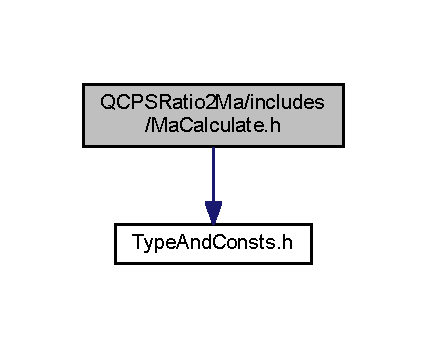
\includegraphics[width=205pt]{_ma_calculate_8h__incl}
\end{center}
\end{figure}
此图展示该文件直接或间接的被哪些文件引用了\+:
\nopagebreak
\begin{figure}[H]
\begin{center}
\leavevmode
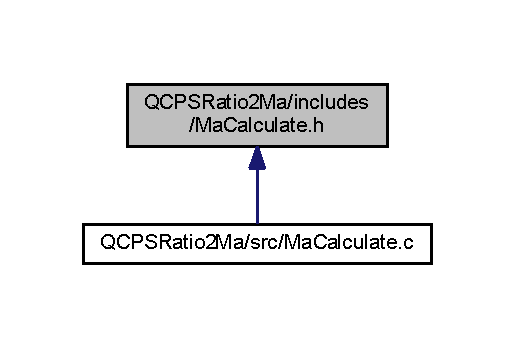
\includegraphics[width=247pt]{_ma_calculate_8h__dep__incl}
\end{center}
\end{figure}
\subsection*{结构体}
\begin{DoxyCompactItemize}
\item 
struct \mbox{\hyperlink{struct_interval}{Interval}}
\begin{DoxyCompactList}\small\item\em 表示一个区间. \end{DoxyCompactList}\end{DoxyCompactItemize}
\subsection*{类型定义}
\begin{DoxyCompactItemize}
\item 
typedef struct \mbox{\hyperlink{struct_interval}{Interval}} \mbox{\hyperlink{_ma_calculate_8h_aaf2b87053de26e4b42b9080f96979381}{Interval}}
\begin{DoxyCompactList}\small\item\em 表示一个区间. \end{DoxyCompactList}\end{DoxyCompactItemize}
\subsection*{函数}
\begin{DoxyCompactItemize}
\item 
\mbox{\hyperlink{_type_and_consts_8h_a3f1431cb9f76da10f59246d1d743dc2c}{Float64}} \mbox{\hyperlink{_ma_calculate_8h_a253892e69f34431bc2545a7c6a3e4d95}{Get\+Ma}} (\mbox{\hyperlink{_type_and_consts_8h_a3f1431cb9f76da10f59246d1d743dc2c}{Float64}} ratio, \mbox{\hyperlink{_type_and_consts_8h_a3f1431cb9f76da10f59246d1d743dc2c}{Float64}} precision)
\begin{DoxyCompactList}\small\item\em 二分法求解马赫数近似值. \end{DoxyCompactList}\item 
\mbox{\hyperlink{_type_and_consts_8h_a3f1431cb9f76da10f59246d1d743dc2c}{Float64}} \mbox{\hyperlink{_ma_calculate_8h_aeb31e4f36a02d9573367a532f6be24af}{Get\+Fn\+Value}} (\mbox{\hyperlink{_type_and_consts_8h_a3f1431cb9f76da10f59246d1d743dc2c}{Float64}} Ma, \mbox{\hyperlink{_type_and_consts_8h_a3f1431cb9f76da10f59246d1d743dc2c}{Float64}} ratio)
\begin{DoxyCompactList}\small\item\em 二分法求解时所用函数,即 f(n) = f(\+Ma) -\/ ratio. \end{DoxyCompactList}\item 
static \mbox{\hyperlink{struct_interval}{Interval}} \mbox{\hyperlink{_ma_calculate_8h_ad2249169f3bdf2640f0b4fe7fdf1f8f5}{Get\+Interval}} (\mbox{\hyperlink{_type_and_consts_8h_a3f1431cb9f76da10f59246d1d743dc2c}{Float64}} ratio)
\item 
static \mbox{\hyperlink{_type_and_consts_8h_adf1ef98b7070177c7c709b0b82276a07}{Int32}} \mbox{\hyperlink{_ma_calculate_8h_a36ec9394e297cfb8a1c715d888e6a785}{If\+Same\+Symbol}} (\mbox{\hyperlink{_type_and_consts_8h_a3f1431cb9f76da10f59246d1d743dc2c}{Float64}} NumA, \mbox{\hyperlink{_type_and_consts_8h_a3f1431cb9f76da10f59246d1d743dc2c}{Float64}} NumB)
\end{DoxyCompactItemize}


\subsection{详细描述}
对\+Ma\+Calculate.\+c中使用的函数及结构体进行声明. 

\begin{DoxyDate}{日期}
2018/9/26. 
\end{DoxyDate}
\begin{DoxyAuthor}{作者}
翟灿 邮箱:840202741.com. 
\end{DoxyAuthor}
\begin{DoxyVersion}{版本}
1.\+0 
\end{DoxyVersion}
\begin{DoxyCopyright}{版权所有}
Copyright © 2018 翟灿. All rights reserved. 
\end{DoxyCopyright}


\subsection{类型定义说明}
\mbox{\Hypertarget{_ma_calculate_8h_aaf2b87053de26e4b42b9080f96979381}\label{_ma_calculate_8h_aaf2b87053de26e4b42b9080f96979381}} 
\index{Ma\+Calculate.\+h@{Ma\+Calculate.\+h}!Interval@{Interval}}
\index{Interval@{Interval}!Ma\+Calculate.\+h@{Ma\+Calculate.\+h}}
\subsubsection{\texorpdfstring{Interval}{Interval}}
{\footnotesize\ttfamily typedef struct \mbox{\hyperlink{struct_interval}{Interval}} \mbox{\hyperlink{struct_interval}{Interval}}}



表示一个区间. 



\subsection{函数说明}
\mbox{\Hypertarget{_ma_calculate_8h_aeb31e4f36a02d9573367a532f6be24af}\label{_ma_calculate_8h_aeb31e4f36a02d9573367a532f6be24af}} 
\index{Ma\+Calculate.\+h@{Ma\+Calculate.\+h}!Get\+Fn\+Value@{Get\+Fn\+Value}}
\index{Get\+Fn\+Value@{Get\+Fn\+Value}!Ma\+Calculate.\+h@{Ma\+Calculate.\+h}}
\subsubsection{\texorpdfstring{Get\+Fn\+Value()}{GetFnValue()}}
{\footnotesize\ttfamily \mbox{\hyperlink{_type_and_consts_8h_a3f1431cb9f76da10f59246d1d743dc2c}{Float64}} Get\+Fn\+Value (\begin{DoxyParamCaption}\item[{\mbox{\hyperlink{_type_and_consts_8h_a3f1431cb9f76da10f59246d1d743dc2c}{Float64}}}]{Ma,  }\item[{\mbox{\hyperlink{_type_and_consts_8h_a3f1431cb9f76da10f59246d1d743dc2c}{Float64}}}]{ratio }\end{DoxyParamCaption})}



二分法求解时所用函数,即 f(n) = f(\+Ma) -\/ ratio. 


\begin{DoxyParams}{参数}
{\em Ma} & 马赫数,单位:无量纲. \\
\hline
{\em ratio} & 动静压比目标值,单位:无量纲. \\
\hline
\end{DoxyParams}
\begin{DoxyReturn}{返回}
动静压比计算值与目标值之差. 
\end{DoxyReturn}
这是这个函数的调用关系图\+:\nopagebreak
\begin{figure}[H]
\begin{center}
\leavevmode
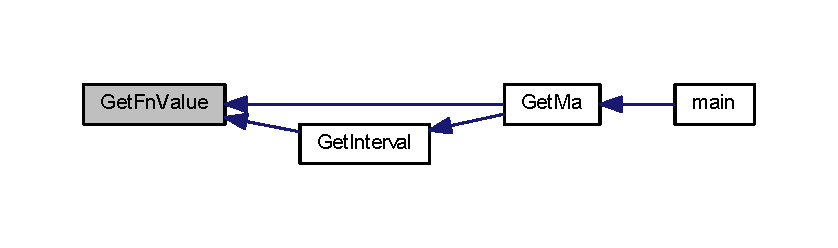
\includegraphics[width=350pt]{_ma_calculate_8h_aeb31e4f36a02d9573367a532f6be24af_icgraph}
\end{center}
\end{figure}
\mbox{\Hypertarget{_ma_calculate_8h_ad2249169f3bdf2640f0b4fe7fdf1f8f5}\label{_ma_calculate_8h_ad2249169f3bdf2640f0b4fe7fdf1f8f5}} 
\index{Ma\+Calculate.\+h@{Ma\+Calculate.\+h}!Get\+Interval@{Get\+Interval}}
\index{Get\+Interval@{Get\+Interval}!Ma\+Calculate.\+h@{Ma\+Calculate.\+h}}
\subsubsection{\texorpdfstring{Get\+Interval()}{GetInterval()}}
{\footnotesize\ttfamily static \mbox{\hyperlink{struct_interval}{Interval}} Get\+Interval (\begin{DoxyParamCaption}\item[{\mbox{\hyperlink{_type_and_consts_8h_a3f1431cb9f76da10f59246d1d743dc2c}{Float64}}}]{ratio }\end{DoxyParamCaption})\hspace{0.3cm}{\ttfamily [static]}}

\mbox{\Hypertarget{_ma_calculate_8h_a253892e69f34431bc2545a7c6a3e4d95}\label{_ma_calculate_8h_a253892e69f34431bc2545a7c6a3e4d95}} 
\index{Ma\+Calculate.\+h@{Ma\+Calculate.\+h}!Get\+Ma@{Get\+Ma}}
\index{Get\+Ma@{Get\+Ma}!Ma\+Calculate.\+h@{Ma\+Calculate.\+h}}
\subsubsection{\texorpdfstring{Get\+Ma()}{GetMa()}}
{\footnotesize\ttfamily \mbox{\hyperlink{_type_and_consts_8h_a3f1431cb9f76da10f59246d1d743dc2c}{Float64}} Get\+Ma (\begin{DoxyParamCaption}\item[{\mbox{\hyperlink{_type_and_consts_8h_a3f1431cb9f76da10f59246d1d743dc2c}{Float64}}}]{ratio,  }\item[{\mbox{\hyperlink{_type_and_consts_8h_a3f1431cb9f76da10f59246d1d743dc2c}{Float64}}}]{precision }\end{DoxyParamCaption})}



二分法求解马赫数近似值. 


\begin{DoxyParams}{参数}
{\em ratio} & 动静压比,单位:无量纲. \\
\hline
{\em precision} & 精确度,推荐值\+:0.\+00001. \\
\hline
\end{DoxyParams}
\begin{DoxyReturn}{返回}
对应的马赫数,单位:无量纲. 
\end{DoxyReturn}
这是这个函数的调用关系图\+:\nopagebreak
\begin{figure}[H]
\begin{center}
\leavevmode
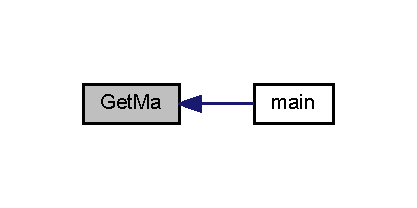
\includegraphics[width=200pt]{_ma_calculate_8h_a253892e69f34431bc2545a7c6a3e4d95_icgraph}
\end{center}
\end{figure}
\mbox{\Hypertarget{_ma_calculate_8h_a36ec9394e297cfb8a1c715d888e6a785}\label{_ma_calculate_8h_a36ec9394e297cfb8a1c715d888e6a785}} 
\index{Ma\+Calculate.\+h@{Ma\+Calculate.\+h}!If\+Same\+Symbol@{If\+Same\+Symbol}}
\index{If\+Same\+Symbol@{If\+Same\+Symbol}!Ma\+Calculate.\+h@{Ma\+Calculate.\+h}}
\subsubsection{\texorpdfstring{If\+Same\+Symbol()}{IfSameSymbol()}}
{\footnotesize\ttfamily static \mbox{\hyperlink{_type_and_consts_8h_adf1ef98b7070177c7c709b0b82276a07}{Int32}} If\+Same\+Symbol (\begin{DoxyParamCaption}\item[{\mbox{\hyperlink{_type_and_consts_8h_a3f1431cb9f76da10f59246d1d743dc2c}{Float64}}}]{NumA,  }\item[{\mbox{\hyperlink{_type_and_consts_8h_a3f1431cb9f76da10f59246d1d743dc2c}{Float64}}}]{NumB }\end{DoxyParamCaption})\hspace{0.3cm}{\ttfamily [static]}}


\hypertarget{main_8h}{}\section{Q\+C\+P\+S\+Ratio2\+Ma/includes/main.h 文件参考}
\label{main_8h}\index{Q\+C\+P\+S\+Ratio2\+Ma/includes/main.\+h@{Q\+C\+P\+S\+Ratio2\+Ma/includes/main.\+h}}


对main.\+c中使用的函数进行声明.  


{\ttfamily \#include \char`\"{}Type\+And\+Consts.\+h\char`\"{}}\newline
main.\+h 的引用(Include)关系图\+:
\nopagebreak
\begin{figure}[H]
\begin{center}
\leavevmode
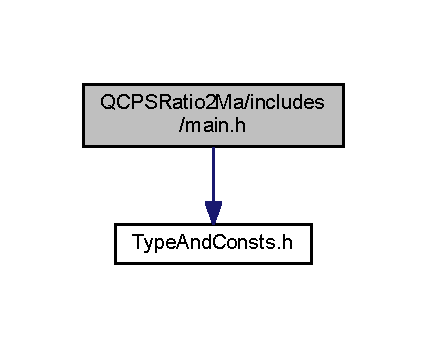
\includegraphics[width=205pt]{main_8h__incl}
\end{center}
\end{figure}
此图展示该文件直接或间接的被哪些文件引用了\+:
\nopagebreak
\begin{figure}[H]
\begin{center}
\leavevmode
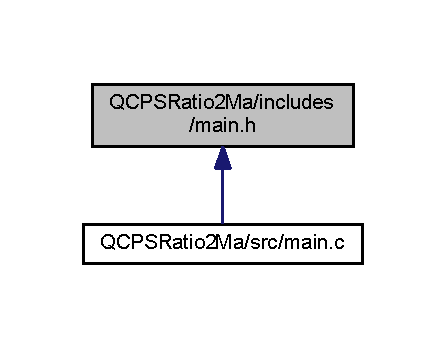
\includegraphics[width=214pt]{main_8h__dep__incl}
\end{center}
\end{figure}
\subsection*{函数}
\begin{DoxyCompactItemize}
\item 
\mbox{\hyperlink{_type_and_consts_8h_a3f1431cb9f76da10f59246d1d743dc2c}{Float64}} \mbox{\hyperlink{main_8h_a253892e69f34431bc2545a7c6a3e4d95}{Get\+Ma}} (\mbox{\hyperlink{_type_and_consts_8h_a3f1431cb9f76da10f59246d1d743dc2c}{Float64}} ratio, \mbox{\hyperlink{_type_and_consts_8h_a3f1431cb9f76da10f59246d1d743dc2c}{Float64}} precision)
\begin{DoxyCompactList}\small\item\em 二分法求解马赫数近似值. \end{DoxyCompactList}\item 
\mbox{\hyperlink{_type_and_consts_8h_a3f1431cb9f76da10f59246d1d743dc2c}{Float64}} \mbox{\hyperlink{main_8h_aa5ab6025b29b45cc2f4099df288c009d}{Get\+Ratio}} (\mbox{\hyperlink{_type_and_consts_8h_a3f1431cb9f76da10f59246d1d743dc2c}{Float64}} Ma)
\begin{DoxyCompactList}\small\item\em 根据马赫数计算动静态气压比. \end{DoxyCompactList}\item 
\mbox{\hyperlink{_type_and_consts_8h_adf1ef98b7070177c7c709b0b82276a07}{Int32}} \mbox{\hyperlink{main_8h_a4934dbfafc20b64a7cc8cdfb395b233c}{main}} (void)
\begin{DoxyCompactList}\small\item\em 程序运行起始函数. \end{DoxyCompactList}\end{DoxyCompactItemize}


\subsection{详细描述}
对main.\+c中使用的函数进行声明. 

\begin{DoxyDate}{日期}
2018/9/26. 
\end{DoxyDate}
\begin{DoxyAuthor}{作者}
翟灿 邮箱:840202741.com. 
\end{DoxyAuthor}
\begin{DoxyVersion}{版本}
1.\+0 
\end{DoxyVersion}
\begin{DoxyCopyright}{版权所有}
Copyright © 2018 翟灿. All rights reserved. 
\end{DoxyCopyright}


\subsection{函数说明}
\mbox{\Hypertarget{main_8h_a253892e69f34431bc2545a7c6a3e4d95}\label{main_8h_a253892e69f34431bc2545a7c6a3e4d95}} 
\index{main.\+h@{main.\+h}!Get\+Ma@{Get\+Ma}}
\index{Get\+Ma@{Get\+Ma}!main.\+h@{main.\+h}}
\subsubsection{\texorpdfstring{Get\+Ma()}{GetMa()}}
{\footnotesize\ttfamily \mbox{\hyperlink{_type_and_consts_8h_a3f1431cb9f76da10f59246d1d743dc2c}{Float64}} Get\+Ma (\begin{DoxyParamCaption}\item[{\mbox{\hyperlink{_type_and_consts_8h_a3f1431cb9f76da10f59246d1d743dc2c}{Float64}}}]{ratio,  }\item[{\mbox{\hyperlink{_type_and_consts_8h_a3f1431cb9f76da10f59246d1d743dc2c}{Float64}}}]{precision }\end{DoxyParamCaption})}



二分法求解马赫数近似值. 


\begin{DoxyParams}{参数}
{\em ratio} & 动静态气压比,单位:无量纲. \\
\hline
{\em precision} & 精确度,推荐值\+:0.\+00001. \\
\hline
\end{DoxyParams}
\begin{DoxyReturn}{返回}
对应的马赫数,单位:无量纲. 
\end{DoxyReturn}
函数调用图\+:
\nopagebreak
\begin{figure}[H]
\begin{center}
\leavevmode
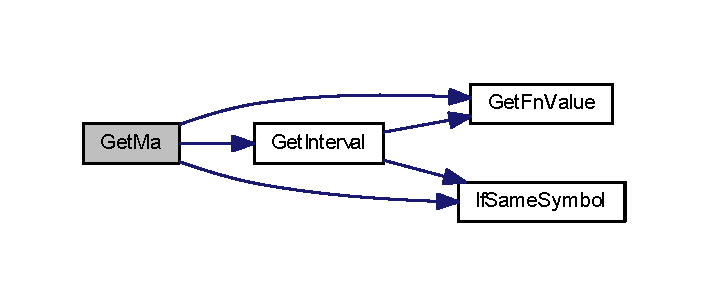
\includegraphics[width=340pt]{main_8h_a253892e69f34431bc2545a7c6a3e4d95_cgraph}
\end{center}
\end{figure}
\mbox{\Hypertarget{main_8h_aa5ab6025b29b45cc2f4099df288c009d}\label{main_8h_aa5ab6025b29b45cc2f4099df288c009d}} 
\index{main.\+h@{main.\+h}!Get\+Ratio@{Get\+Ratio}}
\index{Get\+Ratio@{Get\+Ratio}!main.\+h@{main.\+h}}
\subsubsection{\texorpdfstring{Get\+Ratio()}{GetRatio()}}
{\footnotesize\ttfamily \mbox{\hyperlink{_type_and_consts_8h_a3f1431cb9f76da10f59246d1d743dc2c}{Float64}} Get\+Ratio (\begin{DoxyParamCaption}\item[{\mbox{\hyperlink{_type_and_consts_8h_a3f1431cb9f76da10f59246d1d743dc2c}{Float64}}}]{Ma }\end{DoxyParamCaption})}



根据马赫数计算动静态气压比. 


\begin{DoxyParams}{参数}
{\em Ma} & 马赫数,单位:无量纲. \\
\hline
\end{DoxyParams}
\begin{DoxyReturn}{返回}
马赫数所对应的动静态气压比值,单位:无量纲. 
\end{DoxyReturn}
这是这个函数的调用关系图\+:
\nopagebreak
\begin{figure}[H]
\begin{center}
\leavevmode
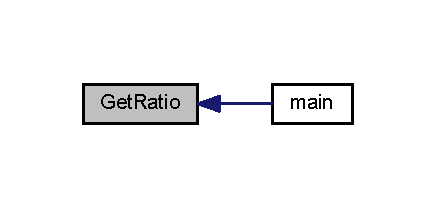
\includegraphics[width=209pt]{main_8h_aa5ab6025b29b45cc2f4099df288c009d_icgraph}
\end{center}
\end{figure}
\mbox{\Hypertarget{main_8h_a4934dbfafc20b64a7cc8cdfb395b233c}\label{main_8h_a4934dbfafc20b64a7cc8cdfb395b233c}} 
\index{main.\+h@{main.\+h}!main@{main}}
\index{main@{main}!main.\+h@{main.\+h}}
\subsubsection{\texorpdfstring{main()}{main()}}
{\footnotesize\ttfamily \mbox{\hyperlink{_type_and_consts_8h_adf1ef98b7070177c7c709b0b82276a07}{Int32}} main (\begin{DoxyParamCaption}\item[{void}]{ }\end{DoxyParamCaption})}



程序运行起始函数. 

函数调用图\+:
\nopagebreak
\begin{figure}[H]
\begin{center}
\leavevmode
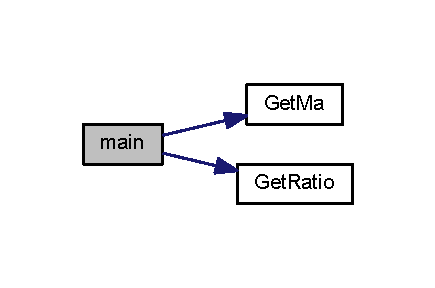
\includegraphics[width=209pt]{main_8h_a4934dbfafc20b64a7cc8cdfb395b233c_cgraph}
\end{center}
\end{figure}

\hypertarget{_ratio_calculate_8h}{}\section{Q\+C\+P\+S\+Ratio2\+Ma/includes/\+Ratio\+Calculate.h 文件参考}
\label{_ratio_calculate_8h}\index{Q\+C\+P\+S\+Ratio2\+Ma/includes/\+Ratio\+Calculate.\+h@{Q\+C\+P\+S\+Ratio2\+Ma/includes/\+Ratio\+Calculate.\+h}}


对\+Ratio\+Calculate.\+c中使用的函数进行声明.  


{\ttfamily \#include \char`\"{}Type\+And\+Consts.\+h\char`\"{}}\newline
Ratio\+Calculate.\+h 的引用(Include)关系图\+:
\nopagebreak
\begin{figure}[H]
\begin{center}
\leavevmode
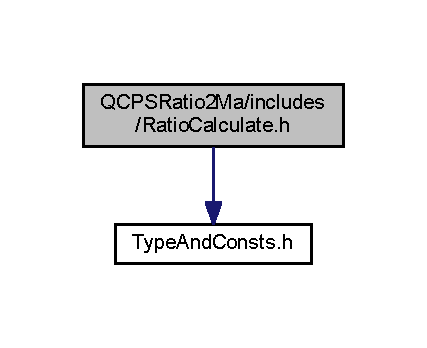
\includegraphics[width=205pt]{_ratio_calculate_8h__incl}
\end{center}
\end{figure}
此图展示该文件直接或间接的被哪些文件引用了\+:
\nopagebreak
\begin{figure}[H]
\begin{center}
\leavevmode
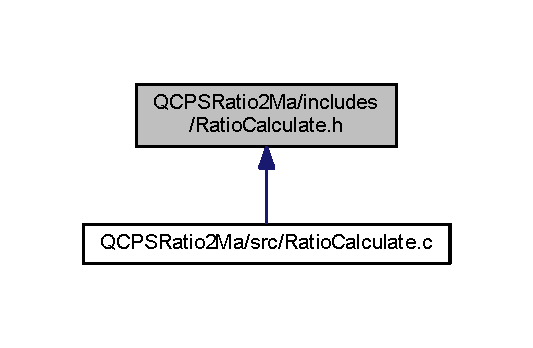
\includegraphics[width=256pt]{_ratio_calculate_8h__dep__incl}
\end{center}
\end{figure}
\subsection*{函数}
\begin{DoxyCompactItemize}
\item 
\mbox{\hyperlink{_type_and_consts_8h_a3f1431cb9f76da10f59246d1d743dc2c}{Float64}} \mbox{\hyperlink{_ratio_calculate_8h_aa5ab6025b29b45cc2f4099df288c009d}{Get\+Ratio}} (\mbox{\hyperlink{_type_and_consts_8h_a3f1431cb9f76da10f59246d1d743dc2c}{Float64}} Ma)
\begin{DoxyCompactList}\small\item\em 根据马赫数计算动静态气压比. \end{DoxyCompactList}\item 
\mbox{\hyperlink{_type_and_consts_8h_a3f1431cb9f76da10f59246d1d743dc2c}{Float64}} \mbox{\hyperlink{_ratio_calculate_8h_aeb31e4f36a02d9573367a532f6be24af}{Get\+Fn\+Value}} (\mbox{\hyperlink{_type_and_consts_8h_a3f1431cb9f76da10f59246d1d743dc2c}{Float64}} Ma, \mbox{\hyperlink{_type_and_consts_8h_a3f1431cb9f76da10f59246d1d743dc2c}{Float64}} ratio)
\begin{DoxyCompactList}\small\item\em 二分法求解时所用函数,即 f(n) = f(\+Ma) -\/ ratio. \end{DoxyCompactList}\end{DoxyCompactItemize}


\subsection{详细描述}
对\+Ratio\+Calculate.\+c中使用的函数进行声明. 

\begin{DoxyDate}{日期}
2018/9/26. 
\end{DoxyDate}
\begin{DoxyAuthor}{作者}
翟灿 邮箱:840202741.com. 
\end{DoxyAuthor}
\begin{DoxyVersion}{版本}
1.\+0 
\end{DoxyVersion}
\begin{DoxyCopyright}{版权所有}
Copyright © 2018 翟灿. All rights reserved. 
\end{DoxyCopyright}


\subsection{函数说明}
\mbox{\Hypertarget{_ratio_calculate_8h_aeb31e4f36a02d9573367a532f6be24af}\label{_ratio_calculate_8h_aeb31e4f36a02d9573367a532f6be24af}} 
\index{Ratio\+Calculate.\+h@{Ratio\+Calculate.\+h}!Get\+Fn\+Value@{Get\+Fn\+Value}}
\index{Get\+Fn\+Value@{Get\+Fn\+Value}!Ratio\+Calculate.\+h@{Ratio\+Calculate.\+h}}
\subsubsection{\texorpdfstring{Get\+Fn\+Value()}{GetFnValue()}}
{\footnotesize\ttfamily \mbox{\hyperlink{_type_and_consts_8h_a3f1431cb9f76da10f59246d1d743dc2c}{Float64}} Get\+Fn\+Value (\begin{DoxyParamCaption}\item[{\mbox{\hyperlink{_type_and_consts_8h_a3f1431cb9f76da10f59246d1d743dc2c}{Float64}}}]{Ma,  }\item[{\mbox{\hyperlink{_type_and_consts_8h_a3f1431cb9f76da10f59246d1d743dc2c}{Float64}}}]{ratio }\end{DoxyParamCaption})}



二分法求解时所用函数,即 f(n) = f(\+Ma) -\/ ratio. 


\begin{DoxyParams}{参数}
{\em Ma} & 马赫数,单位:无量纲. \\
\hline
{\em ratio} & 动静态气压比目标值,单位:无量纲. \\
\hline
\end{DoxyParams}
\begin{DoxyReturn}{返回}
动静态气压比计算值与目标值之差. 
\end{DoxyReturn}
函数调用图\+:
\nopagebreak
\begin{figure}[H]
\begin{center}
\leavevmode
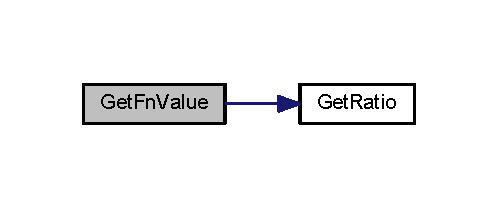
\includegraphics[width=239pt]{_ratio_calculate_8h_aeb31e4f36a02d9573367a532f6be24af_cgraph}
\end{center}
\end{figure}
\mbox{\Hypertarget{_ratio_calculate_8h_aa5ab6025b29b45cc2f4099df288c009d}\label{_ratio_calculate_8h_aa5ab6025b29b45cc2f4099df288c009d}} 
\index{Ratio\+Calculate.\+h@{Ratio\+Calculate.\+h}!Get\+Ratio@{Get\+Ratio}}
\index{Get\+Ratio@{Get\+Ratio}!Ratio\+Calculate.\+h@{Ratio\+Calculate.\+h}}
\subsubsection{\texorpdfstring{Get\+Ratio()}{GetRatio()}}
{\footnotesize\ttfamily \mbox{\hyperlink{_type_and_consts_8h_a3f1431cb9f76da10f59246d1d743dc2c}{Float64}} Get\+Ratio (\begin{DoxyParamCaption}\item[{\mbox{\hyperlink{_type_and_consts_8h_a3f1431cb9f76da10f59246d1d743dc2c}{Float64}}}]{Ma }\end{DoxyParamCaption})}



根据马赫数计算动静态气压比. 


\begin{DoxyParams}{参数}
{\em Ma} & 马赫数,单位:无量纲. \\
\hline
\end{DoxyParams}
\begin{DoxyReturn}{返回}
马赫数所对应的动静态气压比值,单位:无量纲. 
\end{DoxyReturn}
这是这个函数的调用关系图\+:
\nopagebreak
\begin{figure}[H]
\begin{center}
\leavevmode
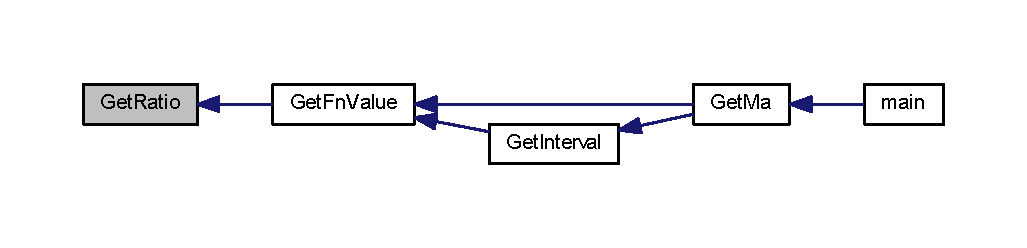
\includegraphics[width=350pt]{_ratio_calculate_8h_aa5ab6025b29b45cc2f4099df288c009d_icgraph}
\end{center}
\end{figure}

\hypertarget{_type_and_consts_8h}{}\section{Q\+C\+P\+S\+Ratio2\+Ma/includes/\+Type\+And\+Consts.h 文件参考}
\label{_type_and_consts_8h}\index{Q\+C\+P\+S\+Ratio2\+Ma/includes/\+Type\+And\+Consts.\+h@{Q\+C\+P\+S\+Ratio2\+Ma/includes/\+Type\+And\+Consts.\+h}}


定义类型及常数.  


此图展示该文件直接或间接的被哪些文件引用了\+:
\nopagebreak
\begin{figure}[H]
\begin{center}
\leavevmode
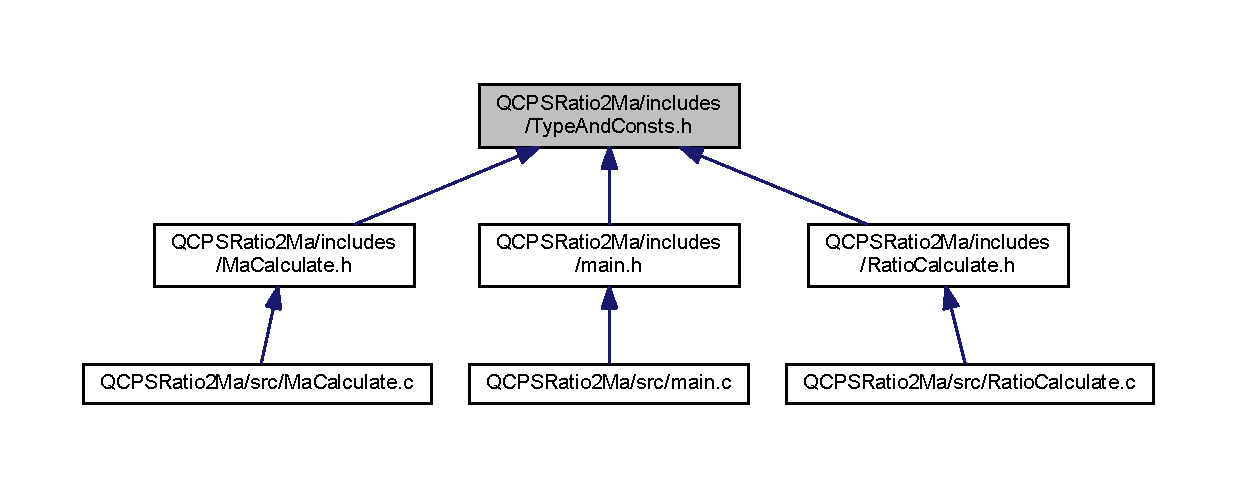
\includegraphics[width=350pt]{_type_and_consts_8h__dep__incl}
\end{center}
\end{figure}
\subsection*{宏定义}
\begin{DoxyCompactItemize}
\item 
\#define \mbox{\hyperlink{_type_and_consts_8h_a1e734b9cf13e77f7f0910fc0b3ce6cf9}{Kn}}~(1.\+4)
\begin{DoxyCompactList}\small\item\em 绝热指数,单位:无量纲 \end{DoxyCompactList}\end{DoxyCompactItemize}
\subsection*{类型定义}
\begin{DoxyCompactItemize}
\item 
typedef int \mbox{\hyperlink{_type_and_consts_8h_adf1ef98b7070177c7c709b0b82276a07}{Int32}}
\begin{DoxyCompactList}\small\item\em 32位整型数 \end{DoxyCompactList}\item 
typedef double \mbox{\hyperlink{_type_and_consts_8h_a3f1431cb9f76da10f59246d1d743dc2c}{Float64}}
\begin{DoxyCompactList}\small\item\em 64位浮点型数 \end{DoxyCompactList}\end{DoxyCompactItemize}


\subsection{详细描述}
定义类型及常数. 

\begin{DoxyDate}{日期}
2018/9/26. 
\end{DoxyDate}
\begin{DoxyAuthor}{作者}
翟灿 邮箱:840202741.com. 
\end{DoxyAuthor}
\begin{DoxyVersion}{版本}
1.\+0 
\end{DoxyVersion}
\begin{DoxyCopyright}{版权所有}
Copyright © 2018 翟灿. All rights reserved. 
\end{DoxyCopyright}


\subsection{宏定义说明}
\mbox{\Hypertarget{_type_and_consts_8h_a1e734b9cf13e77f7f0910fc0b3ce6cf9}\label{_type_and_consts_8h_a1e734b9cf13e77f7f0910fc0b3ce6cf9}} 
\index{Type\+And\+Consts.\+h@{Type\+And\+Consts.\+h}!Kn@{Kn}}
\index{Kn@{Kn}!Type\+And\+Consts.\+h@{Type\+And\+Consts.\+h}}
\subsubsection{\texorpdfstring{Kn}{Kn}}
{\footnotesize\ttfamily \#define Kn~(1.\+4)}



绝热指数,单位:无量纲 



\subsection{类型定义说明}
\mbox{\Hypertarget{_type_and_consts_8h_a3f1431cb9f76da10f59246d1d743dc2c}\label{_type_and_consts_8h_a3f1431cb9f76da10f59246d1d743dc2c}} 
\index{Type\+And\+Consts.\+h@{Type\+And\+Consts.\+h}!Float64@{Float64}}
\index{Float64@{Float64}!Type\+And\+Consts.\+h@{Type\+And\+Consts.\+h}}
\subsubsection{\texorpdfstring{Float64}{Float64}}
{\footnotesize\ttfamily typedef double \mbox{\hyperlink{_type_and_consts_8h_a3f1431cb9f76da10f59246d1d743dc2c}{Float64}}}



64位浮点型数 

\mbox{\Hypertarget{_type_and_consts_8h_adf1ef98b7070177c7c709b0b82276a07}\label{_type_and_consts_8h_adf1ef98b7070177c7c709b0b82276a07}} 
\index{Type\+And\+Consts.\+h@{Type\+And\+Consts.\+h}!Int32@{Int32}}
\index{Int32@{Int32}!Type\+And\+Consts.\+h@{Type\+And\+Consts.\+h}}
\subsubsection{\texorpdfstring{Int32}{Int32}}
{\footnotesize\ttfamily typedef int \mbox{\hyperlink{_type_and_consts_8h_adf1ef98b7070177c7c709b0b82276a07}{Int32}}}



32位整型数 


\hypertarget{_ma_calculate_8c}{}\section{Q\+C\+P\+S\+Ratio2\+Ma/src/\+Ma\+Calculate.c 文件参考}
\label{_ma_calculate_8c}\index{Q\+C\+P\+S\+Ratio2\+Ma/src/\+Ma\+Calculate.\+c@{Q\+C\+P\+S\+Ratio2\+Ma/src/\+Ma\+Calculate.\+c}}


根据动静压比计算马赫数.  


{\ttfamily \#include $<$stdio.\+h$>$}\newline
{\ttfamily \#include $<$math.\+h$>$}\newline
{\ttfamily \#include \char`\"{}Ma\+Calculate.\+h\char`\"{}}\newline
Ma\+Calculate.\+c 的引用(Include)关系图\+:\nopagebreak
\begin{figure}[H]
\begin{center}
\leavevmode
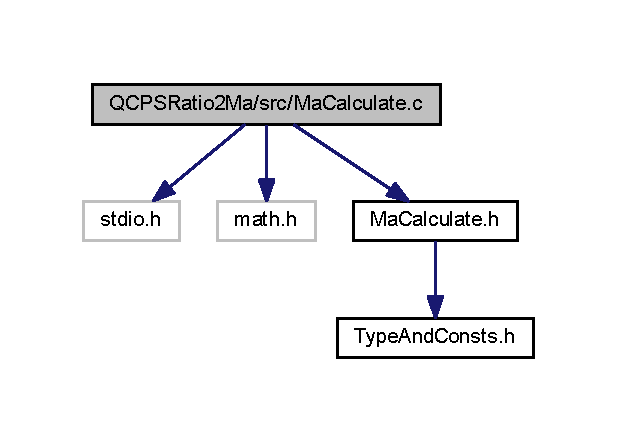
\includegraphics[width=296pt]{_ma_calculate_8c__incl}
\end{center}
\end{figure}
\subsection*{函数}
\begin{DoxyCompactItemize}
\item 
\mbox{\hyperlink{_type_and_consts_8h_a3f1431cb9f76da10f59246d1d743dc2c}{Float64}} \mbox{\hyperlink{_ma_calculate_8c_a253892e69f34431bc2545a7c6a3e4d95}{Get\+Ma}} (\mbox{\hyperlink{_type_and_consts_8h_a3f1431cb9f76da10f59246d1d743dc2c}{Float64}} ratio, \mbox{\hyperlink{_type_and_consts_8h_a3f1431cb9f76da10f59246d1d743dc2c}{Float64}} precision)
\begin{DoxyCompactList}\small\item\em 二分法求解马赫数近似值. \end{DoxyCompactList}\item 
static \mbox{\hyperlink{struct_interval}{Interval}} \mbox{\hyperlink{_ma_calculate_8c_ad2249169f3bdf2640f0b4fe7fdf1f8f5}{Get\+Interval}} (\mbox{\hyperlink{_type_and_consts_8h_a3f1431cb9f76da10f59246d1d743dc2c}{Float64}} ratio)
\begin{DoxyCompactList}\small\item\em 寻找根值所在区间. \end{DoxyCompactList}\item 
static \mbox{\hyperlink{_type_and_consts_8h_adf1ef98b7070177c7c709b0b82276a07}{Int32}} \mbox{\hyperlink{_ma_calculate_8c_a36ec9394e297cfb8a1c715d888e6a785}{If\+Same\+Symbol}} (\mbox{\hyperlink{_type_and_consts_8h_a3f1431cb9f76da10f59246d1d743dc2c}{Float64}} NumA, \mbox{\hyperlink{_type_and_consts_8h_a3f1431cb9f76da10f59246d1d743dc2c}{Float64}} NumB)
\begin{DoxyCompactList}\small\item\em 判断两个数同号还是异号. \end{DoxyCompactList}\end{DoxyCompactItemize}


\subsection{详细描述}
根据动静压比计算马赫数. 

\begin{DoxyDate}{日期}
2018/9/26. 
\end{DoxyDate}
\begin{DoxyAuthor}{作者}
翟灿 邮箱:840202741.com. 
\end{DoxyAuthor}
\begin{DoxyVersion}{版本}
1.\+0 
\end{DoxyVersion}
\begin{DoxyCopyright}{版权所有}
Copyright © 2018 翟灿. All rights reserved. 
\end{DoxyCopyright}


\subsection{函数说明}
\mbox{\Hypertarget{_ma_calculate_8c_ad2249169f3bdf2640f0b4fe7fdf1f8f5}\label{_ma_calculate_8c_ad2249169f3bdf2640f0b4fe7fdf1f8f5}} 
\index{Ma\+Calculate.\+c@{Ma\+Calculate.\+c}!Get\+Interval@{Get\+Interval}}
\index{Get\+Interval@{Get\+Interval}!Ma\+Calculate.\+c@{Ma\+Calculate.\+c}}
\subsubsection{\texorpdfstring{Get\+Interval()}{GetInterval()}}
{\footnotesize\ttfamily static \mbox{\hyperlink{struct_interval}{Interval}} Get\+Interval (\begin{DoxyParamCaption}\item[{\mbox{\hyperlink{_type_and_consts_8h_a3f1431cb9f76da10f59246d1d743dc2c}{Float64}}}]{ratio }\end{DoxyParamCaption})\hspace{0.3cm}{\ttfamily [static]}}



寻找根值所在区间. 


\begin{DoxyParams}{参数}
{\em ratio} & 动静压比,单位:无量纲. \\
\hline
\end{DoxyParams}
\begin{DoxyReturn}{返回}
根值所在区间. 
\end{DoxyReturn}
函数调用图\+:\nopagebreak
\begin{figure}[H]
\begin{center}
\leavevmode
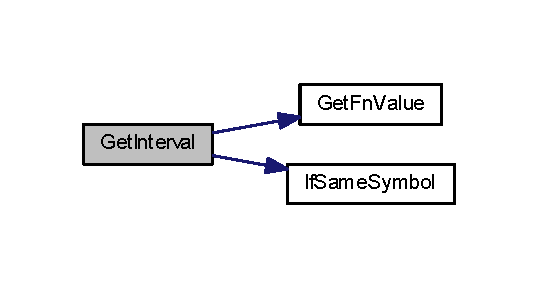
\includegraphics[width=258pt]{_ma_calculate_8c_ad2249169f3bdf2640f0b4fe7fdf1f8f5_cgraph}
\end{center}
\end{figure}
这是这个函数的调用关系图\+:\nopagebreak
\begin{figure}[H]
\begin{center}
\leavevmode
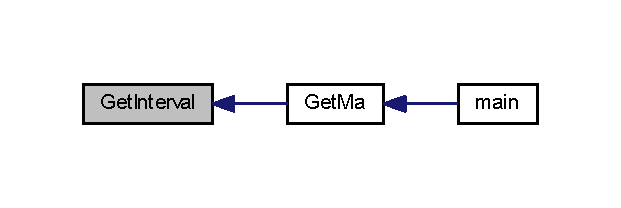
\includegraphics[width=298pt]{_ma_calculate_8c_ad2249169f3bdf2640f0b4fe7fdf1f8f5_icgraph}
\end{center}
\end{figure}
\mbox{\Hypertarget{_ma_calculate_8c_a253892e69f34431bc2545a7c6a3e4d95}\label{_ma_calculate_8c_a253892e69f34431bc2545a7c6a3e4d95}} 
\index{Ma\+Calculate.\+c@{Ma\+Calculate.\+c}!Get\+Ma@{Get\+Ma}}
\index{Get\+Ma@{Get\+Ma}!Ma\+Calculate.\+c@{Ma\+Calculate.\+c}}
\subsubsection{\texorpdfstring{Get\+Ma()}{GetMa()}}
{\footnotesize\ttfamily \mbox{\hyperlink{_type_and_consts_8h_a3f1431cb9f76da10f59246d1d743dc2c}{Float64}} Get\+Ma (\begin{DoxyParamCaption}\item[{\mbox{\hyperlink{_type_and_consts_8h_a3f1431cb9f76da10f59246d1d743dc2c}{Float64}}}]{ratio,  }\item[{\mbox{\hyperlink{_type_and_consts_8h_a3f1431cb9f76da10f59246d1d743dc2c}{Float64}}}]{precision }\end{DoxyParamCaption})}



二分法求解马赫数近似值. 


\begin{DoxyParams}{参数}
{\em ratio} & 动静压比,单位:无量纲. \\
\hline
{\em precision} & 精确度,推荐值\+:0.\+00001. \\
\hline
\end{DoxyParams}
\begin{DoxyReturn}{返回}
对应的马赫数,单位:无量纲. 
\end{DoxyReturn}
函数调用图\+:\nopagebreak
\begin{figure}[H]
\begin{center}
\leavevmode
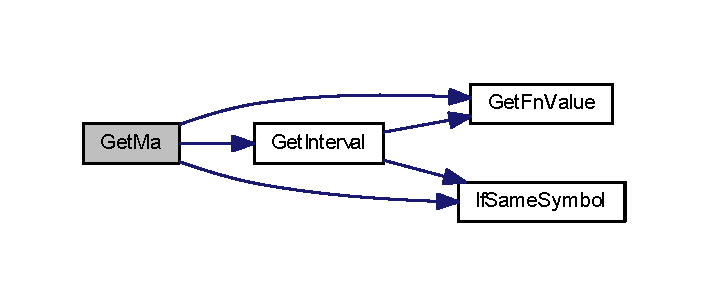
\includegraphics[width=340pt]{_ma_calculate_8c_a253892e69f34431bc2545a7c6a3e4d95_cgraph}
\end{center}
\end{figure}
这是这个函数的调用关系图\+:\nopagebreak
\begin{figure}[H]
\begin{center}
\leavevmode
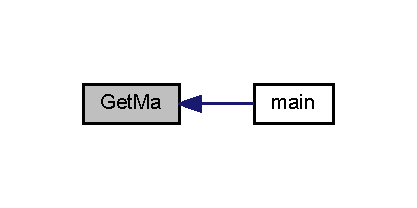
\includegraphics[width=200pt]{_ma_calculate_8c_a253892e69f34431bc2545a7c6a3e4d95_icgraph}
\end{center}
\end{figure}
\mbox{\Hypertarget{_ma_calculate_8c_a36ec9394e297cfb8a1c715d888e6a785}\label{_ma_calculate_8c_a36ec9394e297cfb8a1c715d888e6a785}} 
\index{Ma\+Calculate.\+c@{Ma\+Calculate.\+c}!If\+Same\+Symbol@{If\+Same\+Symbol}}
\index{If\+Same\+Symbol@{If\+Same\+Symbol}!Ma\+Calculate.\+c@{Ma\+Calculate.\+c}}
\subsubsection{\texorpdfstring{If\+Same\+Symbol()}{IfSameSymbol()}}
{\footnotesize\ttfamily static \mbox{\hyperlink{_type_and_consts_8h_adf1ef98b7070177c7c709b0b82276a07}{Int32}} If\+Same\+Symbol (\begin{DoxyParamCaption}\item[{\mbox{\hyperlink{_type_and_consts_8h_a3f1431cb9f76da10f59246d1d743dc2c}{Float64}}}]{NumA,  }\item[{\mbox{\hyperlink{_type_and_consts_8h_a3f1431cb9f76da10f59246d1d743dc2c}{Float64}}}]{NumB }\end{DoxyParamCaption})\hspace{0.3cm}{\ttfamily [static]}}



判断两个数同号还是异号. 


\begin{DoxyParams}{参数}
{\em NumA} & 数字A. \\
\hline
{\em NumB} & 数字B. \\
\hline
\end{DoxyParams}

\begin{DoxyRetVals}{返回值}
{\em 1} & 两个数同号. \\
\hline
{\em 0} & 两个数异号(此处0和0看作异号). \\
\hline
\end{DoxyRetVals}
这是这个函数的调用关系图\+:\nopagebreak
\begin{figure}[H]
\begin{center}
\leavevmode
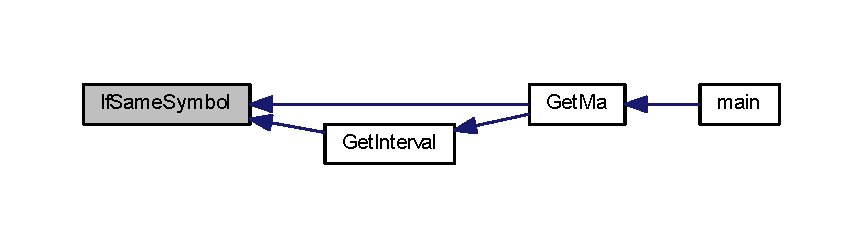
\includegraphics[width=350pt]{_ma_calculate_8c_a36ec9394e297cfb8a1c715d888e6a785_icgraph}
\end{center}
\end{figure}

\hypertarget{main_8c}{}\section{Q\+C\+P\+S\+Ratio2\+Ma/src/main.c 文件参考}
\label{main_8c}\index{Q\+C\+P\+S\+Ratio2\+Ma/src/main.\+c@{Q\+C\+P\+S\+Ratio2\+Ma/src/main.\+c}}


程序运行起始文件.  


{\ttfamily \#include $<$stdio.\+h$>$}\newline
{\ttfamily \#include $<$stdlib.\+h$>$}\newline
{\ttfamily \#include \char`\"{}main.\+h\char`\"{}}\newline
main.\+c 的引用(Include)关系图\+:\nopagebreak
\begin{figure}[H]
\begin{center}
\leavevmode
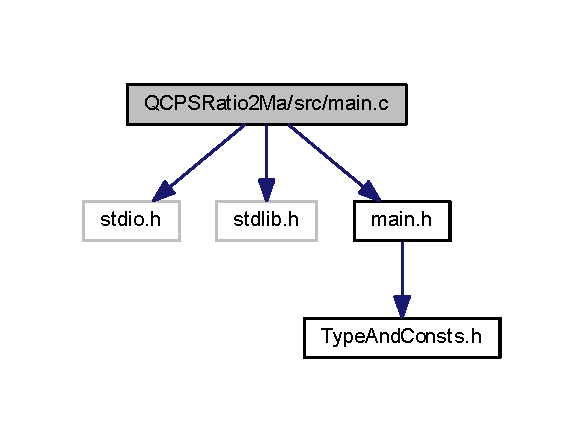
\includegraphics[width=280pt]{main_8c__incl}
\end{center}
\end{figure}
\subsection*{函数}
\begin{DoxyCompactItemize}
\item 
\mbox{\hyperlink{_type_and_consts_8h_adf1ef98b7070177c7c709b0b82276a07}{Int32}} \mbox{\hyperlink{main_8c_a4934dbfafc20b64a7cc8cdfb395b233c}{main}} (void)
\begin{DoxyCompactList}\small\item\em 程序运行起始函数. \end{DoxyCompactList}\end{DoxyCompactItemize}


\subsection{详细描述}
程序运行起始文件. 

\begin{DoxyDate}{日期}
2018/9/26. 
\end{DoxyDate}
\begin{DoxyAuthor}{作者}
翟灿 邮箱:840202741.com. 
\end{DoxyAuthor}
\begin{DoxyVersion}{版本}
1.\+0 
\end{DoxyVersion}
\begin{DoxyCopyright}{版权所有}
Copyright © 2018 翟灿. All rights reserved. 
\end{DoxyCopyright}


\subsection{函数说明}
\mbox{\Hypertarget{main_8c_a4934dbfafc20b64a7cc8cdfb395b233c}\label{main_8c_a4934dbfafc20b64a7cc8cdfb395b233c}} 
\index{main.\+c@{main.\+c}!main@{main}}
\index{main@{main}!main.\+c@{main.\+c}}
\subsubsection{\texorpdfstring{main()}{main()}}
{\footnotesize\ttfamily \mbox{\hyperlink{_type_and_consts_8h_adf1ef98b7070177c7c709b0b82276a07}{Int32}} main (\begin{DoxyParamCaption}\item[{void}]{ }\end{DoxyParamCaption})}



程序运行起始函数. 

函数调用图\+:
\nopagebreak
\begin{figure}[H]
\begin{center}
\leavevmode
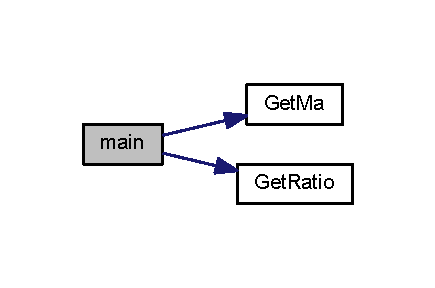
\includegraphics[width=209pt]{main_8c_a4934dbfafc20b64a7cc8cdfb395b233c_cgraph}
\end{center}
\end{figure}

\hypertarget{_ratio_calculate_8c}{}\section{Q\+C\+P\+S\+Ratio2\+Ma/src/\+Ratio\+Calculate.c 文件参考}
\label{_ratio_calculate_8c}\index{Q\+C\+P\+S\+Ratio2\+Ma/src/\+Ratio\+Calculate.\+c@{Q\+C\+P\+S\+Ratio2\+Ma/src/\+Ratio\+Calculate.\+c}}


计算动静压比值.  


{\ttfamily \#include $<$stdio.\+h$>$}\newline
{\ttfamily \#include $<$math.\+h$>$}\newline
{\ttfamily \#include \char`\"{}Ratio\+Calculate.\+h\char`\"{}}\newline
Ratio\+Calculate.\+c 的引用(Include)关系图\+:\nopagebreak
\begin{figure}[H]
\begin{center}
\leavevmode
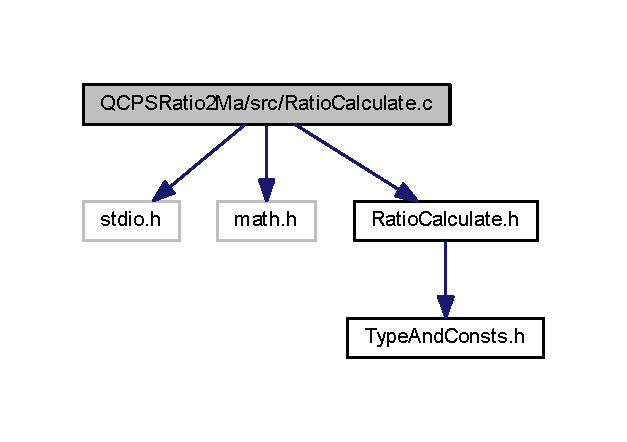
\includegraphics[width=301pt]{_ratio_calculate_8c__incl}
\end{center}
\end{figure}
\subsection*{函数}
\begin{DoxyCompactItemize}
\item 
\mbox{\hyperlink{_type_and_consts_8h_a3f1431cb9f76da10f59246d1d743dc2c}{Float64}} \mbox{\hyperlink{_ratio_calculate_8c_aa5ab6025b29b45cc2f4099df288c009d}{Get\+Ratio}} (\mbox{\hyperlink{_type_and_consts_8h_a3f1431cb9f76da10f59246d1d743dc2c}{Float64}} Ma)
\begin{DoxyCompactList}\small\item\em 根据马赫数计算动静压比. \end{DoxyCompactList}\item 
\mbox{\hyperlink{_type_and_consts_8h_a3f1431cb9f76da10f59246d1d743dc2c}{Float64}} \mbox{\hyperlink{_ratio_calculate_8c_aeb31e4f36a02d9573367a532f6be24af}{Get\+Fn\+Value}} (\mbox{\hyperlink{_type_and_consts_8h_a3f1431cb9f76da10f59246d1d743dc2c}{Float64}} Ma, \mbox{\hyperlink{_type_and_consts_8h_a3f1431cb9f76da10f59246d1d743dc2c}{Float64}} ratio)
\begin{DoxyCompactList}\small\item\em 二分法求解时所用函数,即 f(n) = f(\+Ma) -\/ ratio. \end{DoxyCompactList}\end{DoxyCompactItemize}


\subsection{详细描述}
计算动静压比值. 

\begin{DoxyDate}{日期}
2018/9/26. 
\end{DoxyDate}
\begin{DoxyAuthor}{作者}
翟灿 邮箱:840202741.com. 
\end{DoxyAuthor}
\begin{DoxyVersion}{版本}
1.\+0 
\end{DoxyVersion}
\begin{DoxyCopyright}{版权所有}
Copyright © 2018 翟灿. All rights reserved. 
\end{DoxyCopyright}


\subsection{函数说明}
\mbox{\Hypertarget{_ratio_calculate_8c_aeb31e4f36a02d9573367a532f6be24af}\label{_ratio_calculate_8c_aeb31e4f36a02d9573367a532f6be24af}} 
\index{Ratio\+Calculate.\+c@{Ratio\+Calculate.\+c}!Get\+Fn\+Value@{Get\+Fn\+Value}}
\index{Get\+Fn\+Value@{Get\+Fn\+Value}!Ratio\+Calculate.\+c@{Ratio\+Calculate.\+c}}
\subsubsection{\texorpdfstring{Get\+Fn\+Value()}{GetFnValue()}}
{\footnotesize\ttfamily \mbox{\hyperlink{_type_and_consts_8h_a3f1431cb9f76da10f59246d1d743dc2c}{Float64}} Get\+Fn\+Value (\begin{DoxyParamCaption}\item[{\mbox{\hyperlink{_type_and_consts_8h_a3f1431cb9f76da10f59246d1d743dc2c}{Float64}}}]{Ma,  }\item[{\mbox{\hyperlink{_type_and_consts_8h_a3f1431cb9f76da10f59246d1d743dc2c}{Float64}}}]{ratio }\end{DoxyParamCaption})}



二分法求解时所用函数,即 f(n) = f(\+Ma) -\/ ratio. 


\begin{DoxyParams}{参数}
{\em Ma} & 马赫数,单位:无量纲. \\
\hline
{\em ratio} & 动静压比目标值,单位:无量纲. \\
\hline
\end{DoxyParams}
\begin{DoxyReturn}{返回}
动静压比计算值与目标值之差. 
\end{DoxyReturn}
函数调用图\+:
\nopagebreak
\begin{figure}[H]
\begin{center}
\leavevmode
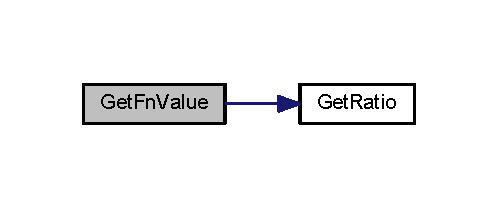
\includegraphics[width=239pt]{_ratio_calculate_8c_aeb31e4f36a02d9573367a532f6be24af_cgraph}
\end{center}
\end{figure}
这是这个函数的调用关系图\+:\nopagebreak
\begin{figure}[H]
\begin{center}
\leavevmode
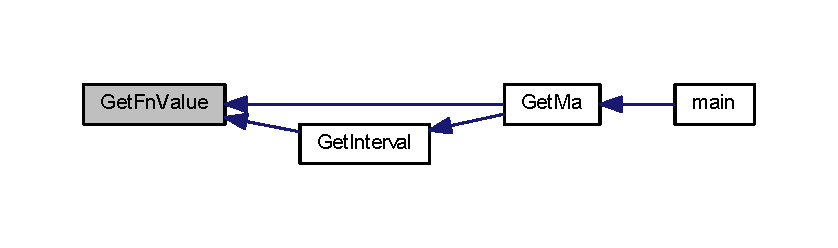
\includegraphics[width=350pt]{_ratio_calculate_8c_aeb31e4f36a02d9573367a532f6be24af_icgraph}
\end{center}
\end{figure}
\mbox{\Hypertarget{_ratio_calculate_8c_aa5ab6025b29b45cc2f4099df288c009d}\label{_ratio_calculate_8c_aa5ab6025b29b45cc2f4099df288c009d}} 
\index{Ratio\+Calculate.\+c@{Ratio\+Calculate.\+c}!Get\+Ratio@{Get\+Ratio}}
\index{Get\+Ratio@{Get\+Ratio}!Ratio\+Calculate.\+c@{Ratio\+Calculate.\+c}}
\subsubsection{\texorpdfstring{Get\+Ratio()}{GetRatio()}}
{\footnotesize\ttfamily \mbox{\hyperlink{_type_and_consts_8h_a3f1431cb9f76da10f59246d1d743dc2c}{Float64}} Get\+Ratio (\begin{DoxyParamCaption}\item[{\mbox{\hyperlink{_type_and_consts_8h_a3f1431cb9f76da10f59246d1d743dc2c}{Float64}}}]{Ma }\end{DoxyParamCaption})}



根据马赫数计算动静压比. 


\begin{DoxyParams}{参数}
{\em Ma} & 马赫数,单位:无量纲. \\
\hline
\end{DoxyParams}
\begin{DoxyReturn}{返回}
马赫数所对应的动静压比值,单位:无量纲. 
\end{DoxyReturn}
这是这个函数的调用关系图\+:\nopagebreak
\begin{figure}[H]
\begin{center}
\leavevmode
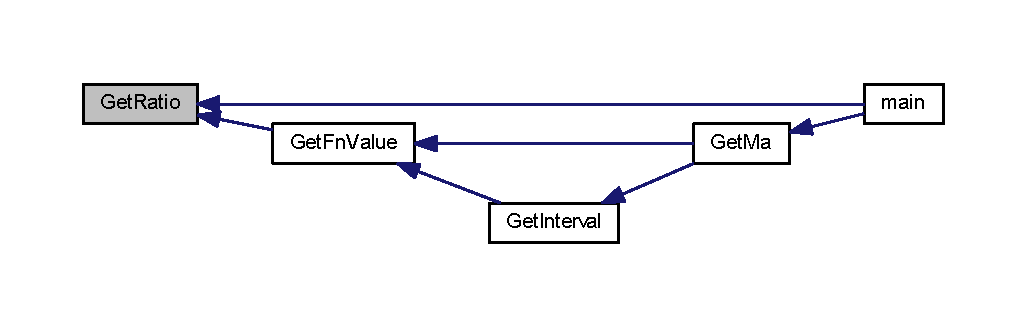
\includegraphics[width=350pt]{_ratio_calculate_8c_aa5ab6025b29b45cc2f4099df288c009d_icgraph}
\end{center}
\end{figure}

%--- End generated contents ---

% Index
\backmatter
\newpage
\phantomsection
\clearemptydoublepage
\addcontentsline{toc}{chapter}{索引}
\printindex

\end{document}
